% =====================================================================
%  DRAFT — AI-ASSISTED TECHNICAL SCAFFOLD, FOR GROUP REVIEW ONLY.
%  Sections 3.2–3.7 of the Execution chapter (Clarence's stream).
%  NOT for verbatim submission: each author must rewrite this in their
%  own words, verify every claim against the code, and replace the
%  \cite{...} placeholders with the group's actual references before the
%  report is submitted. Content is factual (branch clarence/c-block-05,
%  all 14 suites green, 2026-08-14) but the prose must be owned.
%  Requires: \usepackage{booktabs,graphicx}. Tables live in report-tables.tex.
% =====================================================================

\begin{figure}[t]
  \centering
  % convert architecture-two-projections.svg -> .pdf first
  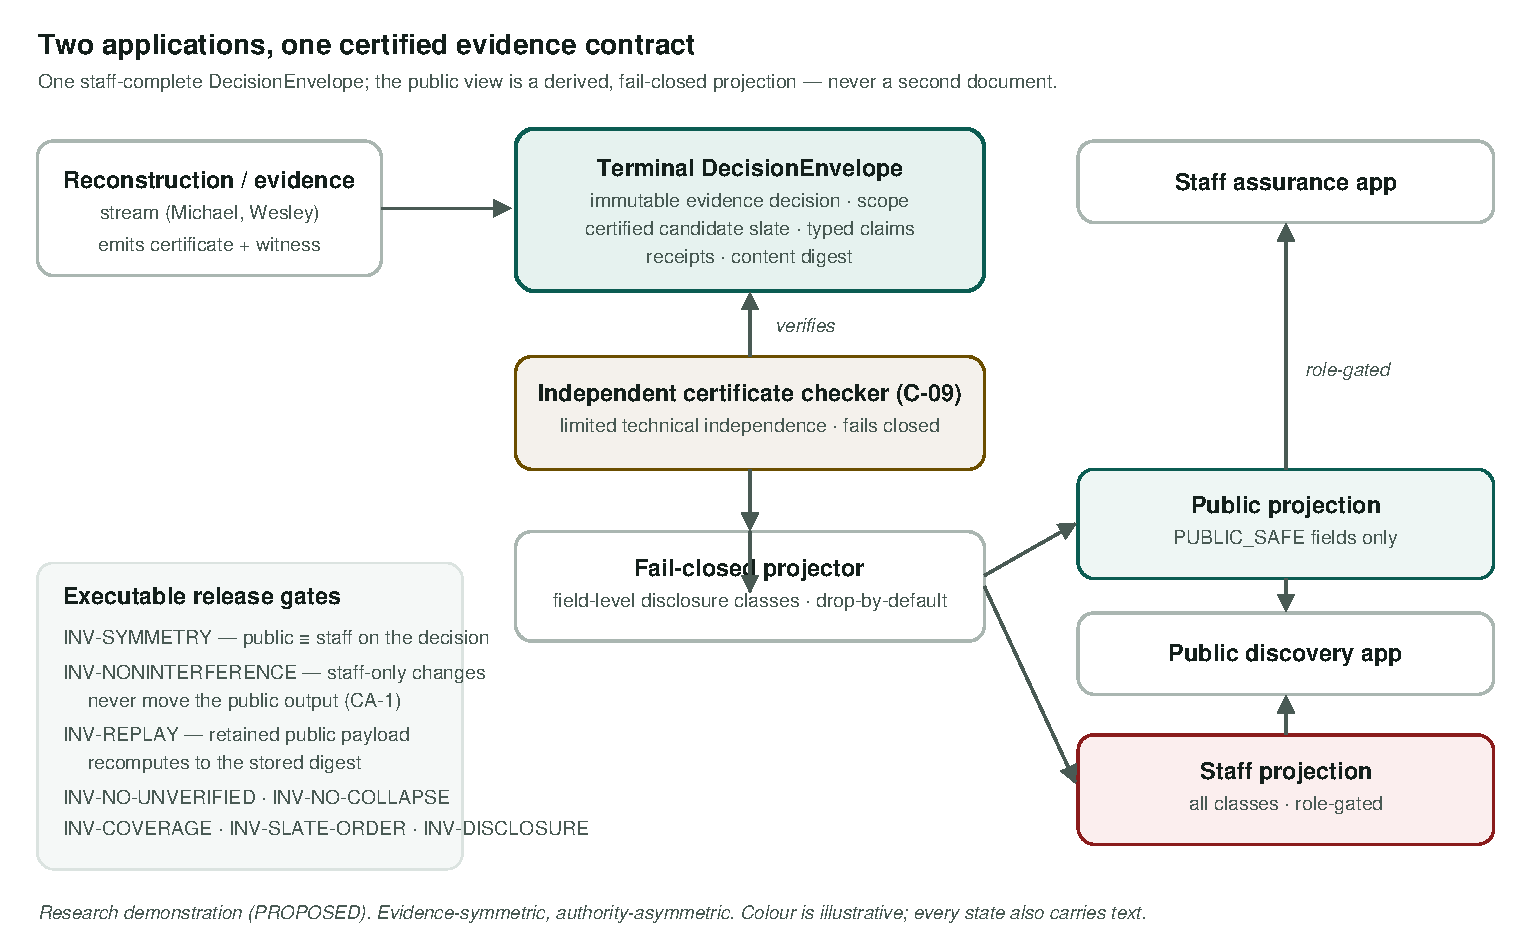
\includegraphics[width=\linewidth]{architecture-two-projections.pdf}
  \caption{One certified evidence contract, two permission-separated projections. The public view is a
  fail-closed projection of the staff-complete \texttt{DecisionEnvelope}; an independent checker
  verifies the decision, and eight executable invariants act as release gates.}
  \label{fig:arch}
\end{figure}

\subsection{Evidence Certification and the Independent Checker}
\label{sec:checker}
A recurring failure mode in evidence-bearing systems is that the component which produces a decision is
also the only component able to attest to it, so that a single implementation fault is both made and
certified in the same place. To avoid this, the architecture separates the production of an evidence
decision from its verification. Alongside each terminal decision, the reconstruction stream emits a
compact certificate and witness; a distinct checker then re-derives whether that certificate is sound.
Rather than run a second, full interpreter---which would roughly double the implementation cost and
could reproduce the very faults it is meant to catch---the checker is built for \emph{limited technical
independence}: it imports no production code, never calls the production interpreter to determine the
expected answer, implements only the frozen certificate contract, and fails closed on anything it
cannot positively verify \cite{selectivepred, groundedgen}. The checker is exercised against the
negative battery summarised in Table~\ref{tab:checker}: thirteen deliberately malformed certificates,
spanning missing or truncated witnesses, swapped and forged receipts, stale and incompatible versions,
an unknown or conflicting state escalated to ``supported'', a dropped scope qualifier, an ineligible
candidate in a supported slate, a certificate issued for a different query, and an ambiguous identity,
are each rejected with a specific outcome code rather than a generic failure. Branch-mutation testing
provides a complementary guarantee: removing each of the eight decision branches in turn produces a
mutant that the suite kills, confirming that no branch is inert. The honest limit of this design is that
its independence is technical rather than external: the author of the checker cannot certify their own
checker, so a non-author code review and a ratified production/reference/checker ownership split remain
outstanding before the control can be relied upon.

\subsection{Conversational Discovery Surface}
\label{sec:chat}
The conversational route is constrained so that language interpretation never becomes factual authority.
Both the guided search and the chat interface resolve to the same terminal \texttt{DecisionEnvelope}, so
that a conversation cannot reach a different answer from the equivalent structured query. The language
model interprets the request and communicates the outcome, but a deterministic verifier authorises every
rendered claim, and no unverified token is streamed to the user; this ``verify-before-render'' ordering
follows from the observation, well established in the grounded-generation and attribution literature,
that fluent text is not itself evidence of truth \cite{groundedgen, attribution}. Three behaviours make
the constraint concrete. High-consequence constraints, such as a stated accessibility need, are
confirmed with the user before any result is shown---a cognitive-forcing step intended to support
appropriate rather than maximal reliance \cite{bucinca2021}. An under-specified request produces a
clarification rather than a fabricated result. And if the model is unavailable, the surface degrades
safely to the guided route rather than guessing. These properties are checked by a conversation test
battery covering convergence, the confirmation gate, clarification, the no-unverified-token rule, and
safe degradation. The current parser is deterministic; a production language model is intended to plug in
behind the same contract, and an adversarial prompt-injection evaluation remains to be carried out.

\subsection{Public Discovery Dashboard}
\label{sec:public}
The public application is server-rendered with a no-JavaScript core, and any client-side enhancement is
layered on top rather than required, so that the core discovery journey remains operable without
scripting; this decision underwrites the accessibility position and the low-bandwidth and no-map routes.
Its defining property is that it renders each evidence state as a distinct outcome rather than collapsing
them into a single ranked list. A supported match, a bounded ``no listed match'' accompanied by a
coverage statement, an indeterminate ``we cannot tell'' state carrying a scope notice, and a safely
degraded service failure are presented as different screens, because a ranked list would hide the very
distinction---between an activity that is absent and one whose data is merely silent---that the system
exists to preserve. Consistent with this, missing information is shown as ``not published'' and never as
``free'' or as a negative fact, so that absence is not converted into false certainty. A comparison view
presents the evidence for each option side by side without declaring a winner. The slice test battery
confirms that every contract state renders, that the public data interface exposes no staff-only fields,
that the wording passes the evidence-language lint, and that ordering is preserved across the evaluation
conditions. The application currently runs over fixed demonstration scenarios and makes no claim to live
availability, booking, or payment.

\subsection{Internal Staff Assurance Dashboard}
\label{sec:staff}
The staff workbench is evidence-symmetric with the public application but authority-asymmetric: it
presents the same certified decision, together with the operational and evidence detail the public plane
must never receive, and it is gated on the server so that a request without a valid role is served no
staff content at all. Access is not granted merely for being a member of staff. A per-role capability
matrix (Table~\ref{tab:roles}) separates viewing and drafting, available to an analyst, from independent
review and approval, available to an assurance role, and from sending, reserved to an authoriser; as a
result the action-card workflow cannot skip independent review, and an action cannot be sent by an
unauthorised role. This is a deliberate separation-of-duties control rather than a cosmetic one. Every
panel additionally carries its provenance---universe, denominator, vintage and versions---and its
permitted wording, and the workbench intentionally offers no league tables and no productivity
monitoring. The staff test battery checks the role gate, evidence symmetry, authority asymmetry (with
internal scores and model versions confirmed to be staff-only), public-state replay, value-level
non-interference, and the send ladder. The role gate is presently a demonstration stub; production
authentication and identity management are a separate work-package and would replace it without altering
the disclosure model.

\subsection{Disclosure Separation and Assurance Controls}
\label{sec:disclosure}
Rather than maintaining separate public and staff schemas that could silently diverge, both surfaces are
derived from a single staff-complete \texttt{DecisionEnvelope} through a fail-closed, class-driven
projection (Figure~\ref{fig:arch}). Every field carries a disclosure class (Table~\ref{tab:disclosure});
the public projection retains only public-safe fields, and any field whose class is not declared is
dropped from every plane by default, so that a newly added field cannot leak through omission. Eight
executable invariants (Table~\ref{tab:invariants}) act as release gates---covering disclosure, value-level
non-interference (a change to a staff-only field cannot alter the public output), evidence symmetry,
semantic replay through a content digest, the prohibition on unverified claims, the prohibition on
collapsing unknown or conflicting states into definite ones, coverage, and slate ordering---and each is
demonstrated both positively, on valid fixtures, and negatively, on adversarial fixtures that the
corresponding gate is required to detect. The value of this discipline was borne out during review, when
the public service-failure page was found to name an internal pipeline stage held in a field that had been
classified as public-safe; the field was reclassified to a staff-only class and a regression test now
prevents its reappearance, which is direct evidence that the controls detect what they are designed to
detect. These guarantees are consolidated in an executable assurance case of fifteen claims
(Table~\ref{tab:assurance}). Its dependency graph is sound and all linked evidence is green; however,
every claim remains blocked pending a named non-author review and an authority decision. This is the
honest maturity state of a research demonstration, and a deliberate refusal to convert ``not yet
reviewed'' into ``authorised''.

\subsection{Accessibility}
\label{sec:a11y}
Accessibility is treated as an evaluation target rather than as a claim to be asserted. The applications
are built \emph{toward} WCAG~2.2~AA within a declared testing matrix, and are not described as conformant
on the strength of an automated scan, because a single examiner-found failure would falsify a blanket
conformance claim whereas a scoped, dated, self-evaluated statement survives scrutiny
\cite{power2012, wcag22}. The no-JavaScript core, a visible focus indicator, minimum target sizes,
automatic light and dark themes, and redundant coding---so that colour is never the sole carrier of
meaning and every evidence state also carries text---are the structural choices made toward that target.
A static accessibility checker is used, but only as one input, and it is not treated as a substitute for
manual keyboard, screen-reader and assistive-technology testing, nor for a review by someone who did not
build the interface. Because that manual and assistive-technology evaluation, and the independent
accessibility review, remain outstanding, the defensible claim is that the applications have been
``evaluated toward WCAG~2.2~AA within the tested matrix'', not that they are ``accessible''.
